\section{Experiments}
\label{sec:results}
We conducted experiments to evaluate the performance of \tmatam  and to compare with the state of the art. 
\subsection{Experimental setup}
\label{subsec:setup}
%\subsubsection{Data}
We employ Twitter's Streaming API to collect tweets between $2014$-Oct-$8$ and $2015$-May-$31$. Collected tweets were subjected to two pre-processing steps as follows.


{\bf Identifying health-related tweets:} We filter the tweets 
returned by the \emph{Decahose Stream} to obtain \emph{health-related} 
tweets. We say that a tweet is health-related if it contains a health 
keyword and passes our classification criteria.  We used 20,000 health-related keywords crawled from
wrongdiagnosis.com to first filter the tweets.
The process is then automated with the help of an SVM classifier~\cite{DBLP:journals/ml/CortesV95}. To this end, $5128$ tweets were 
 annotated through crowdsourcing efforts. The precision and recall of the 
 classifier are $0.85$ and $0.44$. Table~\ref{tab:data:stats} 
shows that out of the 1.36B tweets we collected, 698K were health-related.
\begin{table}[t!]
\centering
\caption{Dataset Statistics}
\label{tab:data:stats}
{\small \begin{tabular}{|c|c|}
\hline
collection period (days) & 235\\
\hline
\#tweets & {1,360,705,803}\\
\hline
\#tweets (health-related) & 698,212\\
\hline
\#tweets (health-related+geolocated) & 569,408\\
\hline
\end{tabular}
}
\end{table}

{\bf Identifying geolocalized tweets:} The ability to operate
seamlessly at varying geographic resolutions mandates that the exact
location of each tweet be known to \tmatam. Twitter affords its users
the option to share their geolocation. In our
case, over half a million tweets are retained ($569K$ as indicated in
Table~\ref{tab:data:stats}).

We examine various choices for the geographic granularities, temporal
granularities and distance measures. \tmatam performs better on
smaller regions. We attribute this
result to the fact that tweets from smaller regions show less diversity in topics. We also found weekly ailment distributions to be very sparse. We also used 2 distance measures to measure distribution difference
namely, cosine similarity and Bhattacharyya distance. We observed that
number of tweets at a given time granularity $t$ may affect the
performance of Cosine Similarity. Finally, we chose to work with geographic granularity of \texttt{\emph{states}}, temporal granularity of \texttt{\emph{months}} and distance measure of \texttt{\emph{Bhattacharyya}}.

{\bf Test-bench and measures:} We run our experiments on a {32 core Intel Xeon @ 2.6Ghz CPU 
(with 20MB cache per core)} system with {128 Gig} RAM running 
{Debian GNU/Linux 7.9 (wheezy)} operating system.
All subsequently discussed components were implemented in 
Java {1.8.0\_60}. 
We used \emph{perplexity} to compare between models \cite{Wallach:2009:EMT:1553374.1553515}.
\subsection{Experimental Results}
Recall that the terms \change and \season refer to the point in time at which discourse density of ailments changes substantially, and the time period before and after that point, respectively. We  divide each \season into training and test sets. \atam is then \emph{\texttt{re-run}} over the training set of each \season. We then model a \transition  \emph{\texttt{$M_{tmatam}^*$}} on the training set of each \season as described in Section~\ref{subsec:model}. We compute the probability of "health topic" $z$ for each tweet $p$ of the first month ($|\mf T|-1$) in the test set using the following formulas:
\begin{equation}
\label{eq:probabilitytopicgiventimepost}
P(z|t_{|\mf T|-1}) = \frac{\sum_{p\ \in t_{|\mf T|-1}}P(z|p\ for\ t_{|\mf T|-1} )}
    {\# tweets\ for\ t_{|\mf T|-1}}
\end{equation}
\begin{equation}
P(z|p)=\sum_{w}P(z|w)P(w|p) = \sum_{w}\frac{n(z,w)}{n(w)}P(w|p)
\end{equation}
Here, values for $n(z,w)$,$n(w)$ are taken from \atam run on the training months. P(w|p) is simply the number of times word $w$ occurs in the tweet $p$ divided by the total number of words in $p$.
We then predict the future probability of each topic in the second month of the test data using the corresponding \transition $M_{tmatam}^*$. Probability of word $p_l(w_i)$ for any document set is calculated as follows:
\begin{equation}
\label{eq:probabilityword}
p_l(w_i)=\sum_{z}P(w|z)P(z) = \sum_{z}\frac{n(z,w)}{n(z)}P(z)
\end{equation}
Having computed $P(w)$, we can compute perplexity against the words of the tweets of second test month.
\subsubsection{\tmatam vs \atam, \tmlda vs \lda}
Figure \ref{fig:perplexity} shows the perplexity ratio of \tmatam with state-of-the art models. If ratio computes to be less than "1" for \competitor, \tmatam is performing worse. If ratio is more than "1" for \competitor, \tmatam is performing better. In order to assert the fact that health topics transit from one to another, we compute the perplexity of \atam on words of the \textit{first month} of the test set and not predicting any topic distribution using any \transition. Hence, this denotes the case where health topics stay \texttt{\emph{static}}. As shown in Figure~\ref{fig:perplexity}, \tmatam beats \atam in all social media active regions (an active region is a region where the proportion of tweets if high enough). For training {\tmlda}, we merge the training data (same as \tmatam) of each \season in each region and train a \transition of \tmlda by solving least squares problem. For each tweet $p$ of the first month of the test set, we compute the probability of topics using LDA trained on merged training data (Formula \ref{eq:probabilitytopicgiventimepost}). We then predict the future probability of each topic in the following month using  $M_{tmlda}^*$. We can then compute the perplexity of \tmlda against words of actual tweets in the test set. Figure~\ref{fig:perplexity} shows that \tmatam consistently beats \tmlda and \lda in predicting future health topics on the test month. Perplexity is indeed lower for all words of the test month in all active states.
\begin{figure}[t!]
\centering
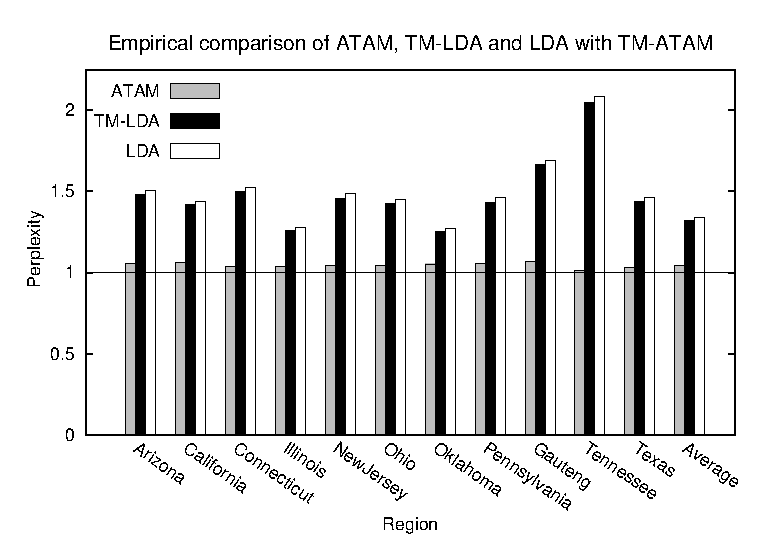
\epsfig{file=gnuplot/perplexity/perplexityRatio2,width=0.45\textwidth}
\caption{Comparison for top 10 active regions. Histograms denote ratio of perplexities. \tmatam is always at 1.0.}  %If ratio is less than "1" for \competitor, \tmatam is performing worse. If ratio is more than "1" for \competitor, \tmatam is performing better.}
\label{fig:perplexity}
\end{figure}
\subsubsection{Homogenous Time Periods}
\label{subsubsec:season}
In Figure \ref{fig:seasonBoundary:NonUS}
we show the top-2 sharpest \changes for the top regions. Those points can be explained with weather
changes in those regions. Texas can be explained with a
drop in temperature while Jervis Bay can be explained by an increase in
rainfall. Dublin sees its lowest temperature in November.
Singapore and Manila have very similar weather conditions and exhibit
the same change point.
\begin{figure}[h!]
\centering
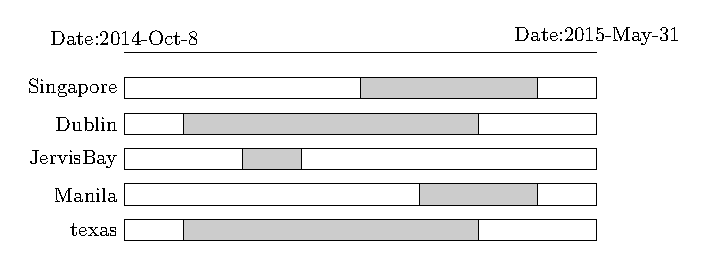
\includegraphics[width=0.45\textwidth]{tikz/seasons_short.pdf}
\caption{Top-2 Monthly \season for top active regions.}
\label{fig:seasonBoundary:NonUS}
\end{figure}
\subsubsection{Topic Transitions}
Entry $m_{ij}$ in the \transition $M$ produced by
\tmatam, shows the degree that topic $z_i$ will contribute to topic $z_j$
in the subsequent \season.
We adapt the threshold used in \cite{DBLP:conf/kdd/WangAB12} to our settings: Threshold  = $\mu + 2\times\sigma_{non-diagonal}$.
We identify two kinds of interesting transitions based on the above threshold:
 \texttt{\emph{selftransitions}}: popular topics and \texttt{\emph{one way transitions}}: $i^{th}$ topic is discussed before $j^{th}$ topic.
As an example, one-way-transitions of California are summarized in Table \ref{tab:fulltransitionCalifornia}.
\begin{table}[t!]
\centering
\caption{One-Way Transitions for California (threshold: $0.815$)}
\label{tab:fulltransitionCalifornia}
{\small \begin{tabular}{|c|c|l|} \hline
 From Topic&To Topic&Weight\\ \hline
  smoking/junkies & respiratory diseases&  2.70\\ /drugs/cigarettes & & \\ \hline
  depression/complaining &  joint pains/body pains&  3.25\\ /cursing/slangs/self-pity & & \\
 \hline\end{tabular} 
}
\end{table}
